% Created 2018-04-24 Tue 21:44
% Intended LaTeX compiler: pdflatex
\documentclass
[
 12pt, % Schriftgröße
       DIV12,
       a4paper,
       oneside,
       titlepage,
       parskip=half,
       headings=normal,
       listof=totoc,
       bibliography=totoc,
       index=totoc,
       captions=tableheading,
       ]{scrreprt}
\input{/Users/dennismuller/dotfiles/networkAssignmentConfig.tex}
\author{Dennis Müller}
\date{\today}
\title{}
\hypersetup{
 pdfauthor={Dennis Müller},
 pdftitle={},
 pdfkeywords={},
 pdfsubject={},
 pdfcreator={Emacs 24.5.1 (Org mode 9.0.5)}, 
 pdflang={English}}
\begin{document}

\tableofcontents


\chapter{Abstract}
\label{sec:org2c9ed28}
\chapter{Introduction}
\label{sec:orgd208c4b}
\section{The Idea}
\label{sec:org210bdc0}

The Digital Life Tracking App is designed to enable users to track their daily tasks and the time spent on them.
To make it more convenient to trigger an activity, the start and end of an activity may be triggered in different ways. 
Possible activation mechanisms could be:
\begin{itemize}
\item Two claps
\item moving the smartphone in a certain way (gestures)
\item activation based on GPS position
\item pressing a button
\end{itemize}

Users should be able to define their own activities and select an activation function from a list and assign it to one of their activities.
The user should then be able to display his history in form of charts.
A separate device (particle photon board) could also be used to trigger a specific activity.

\subsection{The Deep Dive}
\label{sec:org86b9b52}
For the prototype in the context of the assigment we decided to focus mainly on the detection of double clapping as an activity trigger.



\chapter{First Prototype (Board)}
\label{sec:orge6ac6ca}
Explain the state of what we achieved with the board and what problems arised.
\section{Setup}
\label{sec:org493528f}
\begin{itemize}
\item show board setup
\item some code we used
\end{itemize}



\section{Analysis}
\label{sec:org463bcd9}
\begin{itemize}
\item Diagrams that we had in the presentation. Explain problems.
\end{itemize}

Sample rate to low, memory problems, not so easy to debug ( no way of stepping
through code, no UI for giving fast feedback only LEDs)
\section{Conclusion}
\label{sec:org01eb3ff}
move to android.



\chapter{Second Prototype (Android)}
\label{sec:orga08a9a1}

\section{Research for clap detection in android}
\label{sec:org9e5e015}
Java is known to have many open source libraries. For the processing of audio
signals, the Tarsos library was a good choice. Among other things, this offers a
ready-made percussion detection which enables to detect sudden peaks in a
frequency. However, Tarsos also offers more basic functionalities, such as
transforming an audio signal into the frequency domain using Fast Fourier
Transformation.

In order to implement and test the necessary functionality for the state machine
and the UI, the percussions detection from Tarsos was initially used to detect a
loud noise.

\section{Implementation for data analysis}
\label{sec:org56b6177}
Some code was soley written for getting data out of the app and was removed 
later for the final app.

\subsection{Google Drive}
\label{sec:orgee0256e}
When working on the first prototype with the Particle Photon Board, the
roundtrip time required to get the data from the board to a PC, where we can
analyze it, was particularly noticeable. For this reason, an automatic upload of
the CSV data to Google Drive has been implemented. This made it possible to
quickly transfer all recorded data to a central location and analyze it from
there on a PC.
\subsection{CSV Button}
\label{sec:orgf213c4e}
Another functionality that was only necessary for the initial phase is the
recording of the audio signal for a certain period of time and afterwards
writing the transformed (FFT) data into a CSV file.

An extra button was added to the page, which adds a new AudioProcessor to the
AudioDispatcher, which then writes the data to the mobile phone. The existing
CSVWriter class was used and adapted for this.

Unfortunately it turned out that you can't call the method
AudioDispatcherFactory.fromDefaultMicrophone twice to run two dispatchers with
different buffer sizes at the same time. For the recording of test data a longer
period of time is useful over which the FFT is then applied. A buffer size of
3*sampling size was needed, to allow 3 seconds of audio recording per test. For
real application, however, shorter periods of time are needed to detect a double
clap and to keep the delay small.



\section{Implementation}
\label{sec:org8b90d67}
\subsection{Clap Detector}
\label{sec:orgda4522d}
\begin{itemize}
\item Tarsos library ( for FFT )
\end{itemize}
\subsection{State-machine}
\label{sec:org624e913}
A state machine was implemented to represent the different states of the app.
The following diagram shows the implemented state machine.

\begin{center}
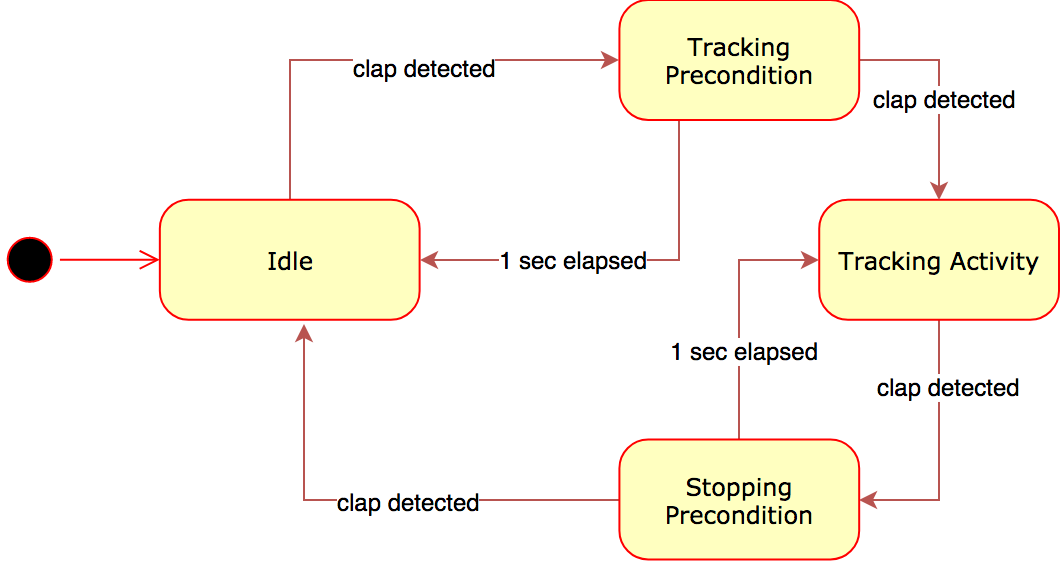
\includegraphics[width=.9\linewidth]{./imgs/statemachine.png}
\end{center}

There are a total of four states in which the app can be in. 
\begin{itemize}
\item Idle: The initial state when starting the app and the state after an activity tracking has been completed.
\item StartPrecondition: If the app is in the idle state and a clap is detected, the state machine switches to this state. When switching to this state, a timer is started which defines the time window in which the second clap must occur in order to switch the state to TrackingActivity. If the timer expires before another clap is detected, the state machine switches back to the idle state.
\item TrackingActivity: After a second clap is detected while the timer of the start precondition has not yet elapsed, the state machine changes to this state and starts capturing the time by saving a time stamp.
\item StoppingPrecondition: If the state machine is in the TrackingActivity state and a clap occurs, then the state machine switches to this state, which behaves in the same way as the StartingPrecondition, except that on a successful second clap, it changes to the idle state and the tracking of the current activity is ended.
\end{itemize}

\subsection{Architecture}
\label{sec:orga3fb9a6}

\begin{center}
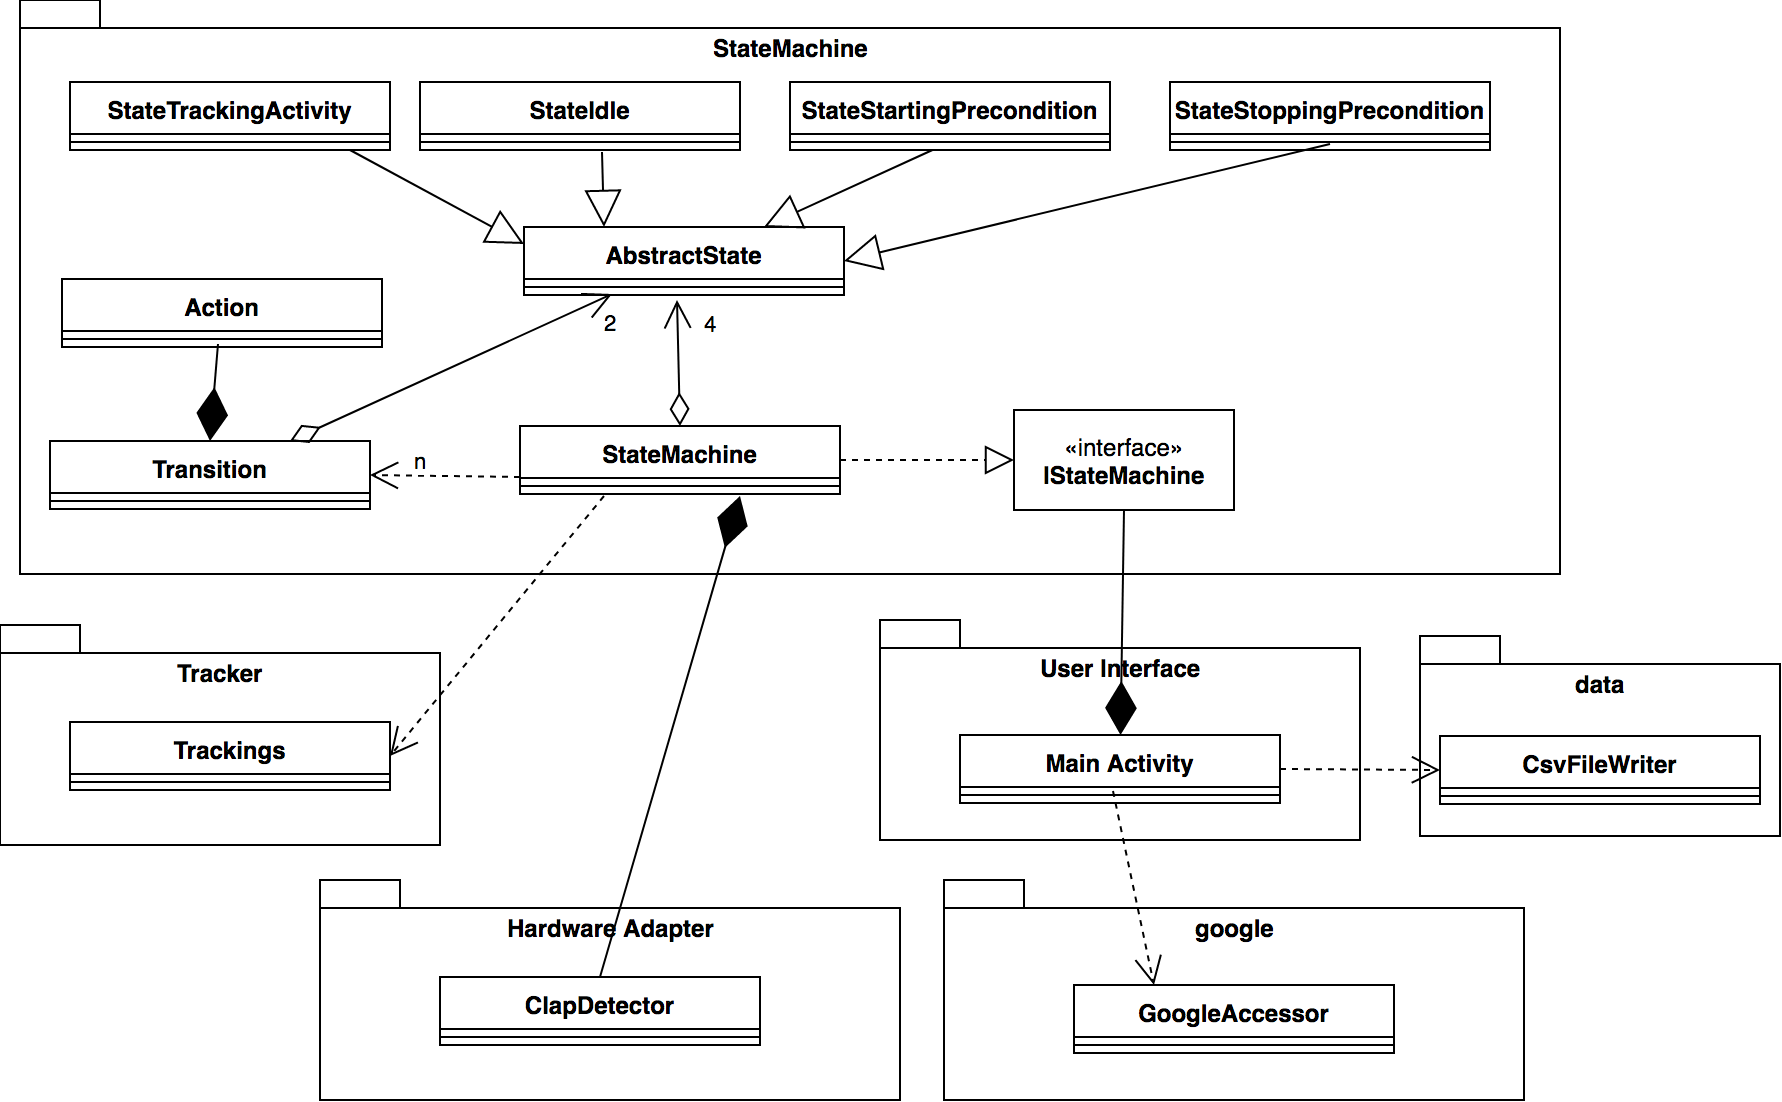
\includegraphics[width=.9\linewidth]{./imgs/classUML.png}
\end{center}

\subsection{UI Design}
\label{sec:orgd655d2f}

\begin{center}
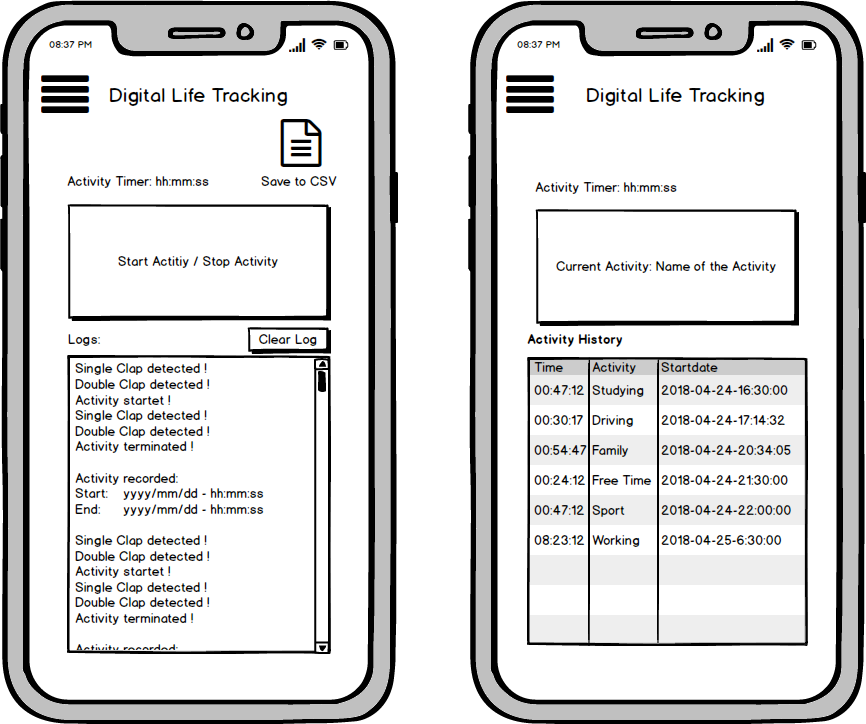
\includegraphics[width=.9\linewidth]{./imgs/mock.png}
\end{center}

\chapter{Conclusion}
\label{sec:org0929265}
\section{Current State}
\label{sec:org6306cc8}
\subsection{Evalutation}
\label{sec:orgeae9f73}
\begin{itemize}
\item How reliable can our implementation detect clap.
\item Benchmark
\begin{itemize}
\item How many time false positives where detected ( 20x husten, 20x schnipsen, 20 klatschen)
\item Show statistics by trying it out (maybe in different environments (loud,
silent rooms, outdoors)
\end{itemize}
\end{itemize}

Refer to to evalution part above. State how difficult this was and the time
needed to try out more advanced solutions (AI) was not enough.

\section{Project Outlook}
\label{sec:orgb2b1f54}
Maybe add more debug functionallity inside the App, be able to not only tweak
parameters inside the code, but also with UI Controls inside the app.

Whistling detection instead of clapping.







\chapter{Referernces}
\label{sec:orgdd19366}
\url{http://www.klangfuzzis.de/showthread.php?679817-Was-hat-in-etwa-wie-viel-hz}

\chapter{Aufgaben für uns noch:}
\label{sec:orgbb94b3e}
\subsection{{\bfseries\sffamily TODO} Tarsos Code rausnkopieren}
\label{sec:orge379dce}
\subsection{{\bfseries\sffamily TODO} State-machine implement}
\label{sec:orga2e3370}
\subsection{{\bfseries\sffamily TODO} Fork vom android und unsere repo reinkopieren}
\label{sec:org7f5b138}
\end{document}